\documentclass{article}
% PACKAGES
\usepackage[english]{babel}
\usepackage{graphicx} % Required for inserting images
\usepackage[most]{tcolorbox}
\usepackage{lmodern}
\usepackage{titlepic}
\usepackage{pdfpages}
\usepackage{tcolorbox}
\usepackage{amsmath}
\usepackage{pgfplots}
\usepackage{xcolor}
\usepackage{tikz}
\usepackage{color,soul}
\usepackage{enumerate}
\usepackage{enumitem}
\usepackage{cancel}
\usepackage{hyperref} 
\usepackage{tikzsymbols}
\usepackage{fontawesome5}
\usepackage[export]{adjustbox}
\usepackage{amssymb}
\usepackage{tikz,lipsum,lmodern}
\usepackage{booktabs}


% COLOURS
\definecolor{Orchid}{RGB}{218, 112, 214}
\definecolor{snow}{rgb}{1.0, 0.98, 0.98}
\definecolor{mordantred19}{rgb}{0.68, 0.05, 0.0}
\definecolor{mistyrose}{rgb}{1.0, 0.89, 0.88}
\definecolor{nadeshikopink}{rgb}{0.96, 0.68, 0.78}
\definecolor{cadmiumgreen}{rgb}{0.0, 0.42, 0.24}
\definecolor{OliveGreen}{RGB}{85, 107, 47}
\definecolor{RoyalPurple}{RGB}{120, 81, 169}
\definecolor{NavyBlue}{RGB}{0, 0, 128}
\definecolor{CornflowerBlue}{RGB}{100, 149, 237}
\definecolor{Cerulean}{RGB}{0, 123, 167}
\definecolor{DarkOrchid}{RGB}{153, 50, 204}

\title{MCV4U - Calculus and Vectors [Chapter 5]}
\author{Kensukeken}
\date{April 4th, 2024}

\begin{document}
\maketitle

\tableofcontents
\newpage
\section{Unit 5 - Derivatives of Exponential and Trigonometric Functions}
\subsection{Trig Derivatives }
The two main rules to remember are the following:
\begin{tcolorbox}[sharp corners=uphill,
    colback=purple!50!white,colframe=blue!25!black,coltext=yellow,
    fontupper=\Large\bfseries,arc=6mm,boxrule=2mm,boxsep=5mm]
$$\frac{\delta (\sin x)}{\delta x}=\cos x \quad \text{and } \quad \frac{\delta(\cos x)}{\delta}=-\sin x$$
\end{tcolorbox}
\textit{Proof} that $\frac{\delta (sin \theta)}{\delta x}=\cos \theta$.\\
We will do this proof in two parts. \\

In the first part, we will prove that  $\lim_{\theta \to 0}\left( \frac{\sin \theta }{\theta}\right)$\\

We need to prove this because it comes up within the main proof, which we will then do in part 2.\\

Part 1: Proving that $\lim_{\theta \to 0}\left( \frac{\sin \theta }{\theta}\right)$\\

Recall that the area of a circle is $\pi r^2=(\frac{2 \pi}{2})r^2$ \\
We will think of our angle $\theta$ in radians \\
The area of the sector of a circle created by a central angle of $\theta$ radians will represent $\frac{\theta}{2\pi}$ of the area of the circle as a whole \\

\begin{minipage}{0.5\textwidth}
For example, if the angle shown is $60^{\circ}$, or $\frac{\pi}{3}$ radians, then the area of the highlighted sector will represent $\left(\frac{\frac{\pi}{3}}{2\pi}\right)=\frac{\pi}{3}\times \frac{1}{2\pi}=\frac{\pi}{6\pi}=\frac{1}{6}$ of the area of the circle as a whole.
\end{minipage}
\hspace{1em}
\begin{minipage}{0.5\textwidth}
\begin{tikzpicture}[scale=2.5] 
\draw (0,0) circle (1cm);
\draw (0,0) -- (0:1cm); 
\draw (0,0) -- (60:1cm); 

\draw (0.2,0) arc (0:60:0.2cm); 
\node at (0.3,0.1) {$\theta$};
\end{tikzpicture}
\end{minipage}

\hspace{1em}


Therefore, for a circle with a radius of r, the area of a sector of that circle created by central angle of $\theta$ radians is given formula \\

\begin{align*}
    \text{Area of Sector} &= \left(\frac{\theta}{2 \oi}\right )(\text{area of circle})\\
    &=\left(\frac{\theta}{2 \pi}\right)(\pi ^2)\\
    &=\left(\frac{\theta}{2}\right)r^2
\end{align*}


Now, focusing on Sector OAB, the length of OB is the radius of the circle from which Sector OAB originates. B and C share the same x-coordinate, as C lies on a vertical line from B. Since C is outside the unit circle, its x-coordinate must be $\cos \theta$. Thus, the radius of the circle from which Sector OAB originates is $\cos \theta$.

As previously stated, the area of a sector is $\left(\frac{\theta}{2}\right)r^2$, and since $r=\cos \theta$, the area of Sector OAB is $\left(\frac{\theta}{2}\right)\cos^2\theta$.

Now, let’s consider Triangle OCB. Its area is $\frac{1}{2}bh$. The base of the triangle is $\cos \theta$, and the height is the y-coordinate of C, which is $\sin \theta$. Thus, the area of Triangle OCB is $\frac{1}{2}\cos \theta \sin \theta$.

Moving to Sector OCD, the area of a sector is $\left(\frac{\theta}{2}\right)r^2$. Since the radius of this sector is 1 (from a unit circle), the area of Sector OCD is $\left(\frac{\theta}{2}\right)(1)^2 = \frac{\theta}{2}$.

Therefore, we have:
\begin{align*}
    &\text{area of Sector OAB is equal to } \left(\frac{\theta}{2} \right)\cos^2\theta\\
    &\text{area of Triangle OCB is } \frac{1}{2}\cos \theta \sin \theta \\
    &\text{area of Sector OCD is } \frac{\theta}{2}
\end{align*}


Putting together the statement above and the statement to the right, we get
\begin{equation*}
    \left(\frac{\theta}{2} \right)\cos^2\theta \leq \frac{1}{2}\cos \theta \sin \theta \leq \frac{\theta}{2}
\end{equation*}

Next, we multiplying the left middle and right by $\frac{2}{\theta \cos \theta}$ gives us 
$$
    \left(\frac{\theta}{2}\right) \cos ^2 \theta \left[\frac{2}{\theta \cos \theta}\right] \leq \frac{1}{2}\cos \theta \sin \theta \left[\frac{2}{\theta \cos \theta}\right] \leq \frac{\theta}{2} \left[\frac{2}{\theta \cos \theta}\right]
$$
$$\cos \theta \leq \frac{\sin \theta}{\theta} \leq \frac{1}{\cos \theta}$$

Determine the limit as $\theta \to 0$ of the left, middle and right
$$\lim_{\theta \to 0}\cos \theta \leq \lim_{\theta \to 0}\frac{\sin \theta}{\theta} \leq \lim_{\theta \to 0}\frac{1}{\cos \theta}$$
We can evaluate the left and the right be simply subbing in a value of $\theta=0$ because those functions are continuous in the neighbourhood around $\theta=0$

\begin{align*}
   & \cos 0 \leq \lim_{\theta \to 0} \frac{\sin \theta}{\theta} \leq \frac{1}{\cos \theta}\\
   & 1 \leq \lim_{\theta \to 0} \frac{\sin \theta}{\theta} \leq \frac{1}{1}\\
   & 1 \leq \lim_{\theta \to 0} \frac{\sin \theta}{\theta} \leq 1
\end{align*}
This next part is really cool, why?\\
The only way that 1 can be both less than or equal to a particular quantity and that the same quantity is less than or equal to 1 is if that quantity is equal to 1.\\
In other words, that quantity is being squeezed so that it’s only possible value is 1

$$\therefore \lim_{\theta \to 0}\frac{\sin \theta}{\theta}=1$$
Part 2:  We needed that result because there will be a moment in our proof that $$\frac{\delta(\sin \theta)}{\delta \theta}=\cos \theta$$ where that value comes up.
\begin{align*}
    \frac{\delta (\sin \theta)}{\delta \theta}&=\lim_{h \to 0}\frac{\sin(\theta+h)-\sin \theta}{h} \text{(next, use compound angle formula)}\\
    &=\lim_{h\to 0}\frac{\sin \theta \cos (h)+\cos \theta \sin(h)-\sin \theta}{h} \text{(next, rearrange the numerator)}\\
    &= \lim_{h\to 0}\frac{\sin \theta \coh (h)-\sin \theta +\cos \theta \sin(h)}{h} \text{(next, split into two fractions)}\\ 
    &=\lim_{h \to 0} \frac{\sin \theta \cos(h)-\sin \theta }{h}+\frac{\cos \theta \sin \theta \sin(h)}{h} \text{(next, factor each numerator)}\\
    &=\lim_{h \to 0} \frac{\sin \theta []\cos (h)-1}{h}+\cos \theta \left(\frac{\sin (h)}{h}\right)\\
    &=\lim_{h \to 0} \sin \theta \left[\frac{\cos (h)-1}{h}\right]+ \cos \theta \left(\frac{\sin (h)}{h}\right)\\    
    &\text{Evaluate the sum of the limits rather than the limit of the sum}\\
    &=\lim_{h \to 0} \sin \theta \left[\frac{\cos (h)-1}{h}\right]+ \lim_{h \to 0}\cos \theta \left(\frac{\sin (h)}{h}\right)\\    
\end{align*}

\newpage 
We can pull $\sin \theta$  in front of the first limit since it’s independent of h and we can pull $\cos \theta$ in front of second limit since it’s also independent of h
$$
\begin{aligned}
& =\sin \theta \lim _{h \rightarrow 0} \frac{\cos (h)-1}{h}+\cos \theta \lim _{h \rightarrow 0} \frac{\sin (h)}{h} \\
& =\sin \theta \lim _{h \rightarrow 0}\left(\frac{\cos (h)-1}{h}\right)\left(\frac{\cos (h)+1}{\cos (h)+1}\right)+\cos \theta \\
& =\sin \theta \lim _{h \rightarrow 0}\left[\frac{\cos ^2 h-1}{h[\cos (h)+1]}\right]+\cos \theta \\
& =\sin \theta \lim _{h \rightarrow 0} \frac{-\sin ^2 h}{h[\cos (h)+1]}+\cos \theta
\end{aligned}
$$
Next, we’ll break apart the fraction of which we are taking the limit:
$$
\begin{aligned}
& =\sin \theta\left[\lim _{h \rightarrow 0}\left(\frac{-\sin (h)}{h} \times \frac{\sin (h)}{\cos (h)+1}\right)\right]+\cos \theta \\
& =\sin \theta\left[\lim _{h \rightarrow 0} \frac{-\sin h}{h} \times \lim _{h \rightarrow 0} \frac{\sin (h)}{\cos (h)+1}\right]+\cos \theta \\
& =\sin \theta\left[-\lim _{h \rightarrow 0} \frac{\sin (h)}{h} \times \lim _{h \rightarrow 0} \frac{\sin (h)}{\cos (h)+1}\right]+\cos \theta \\
& =\sin \theta\left[-(1) \times \frac{\sin 0}{\cos 0+1}\right]+\cos \theta \\
& =\sin \theta\left[-1 \times \frac{0}{1+1}\right]+\cos \theta \\
& =\sin \theta[-1 \times 0]+\cos \theta
\end{aligned}
$$
Consider the product of the limits rather than the limit of the product:
\begin{align*}
    &=\sin[-1\times 0]+\cos\theta\\
    &=(\sin\theta)(0)+\cos \theta\\
    &=\cos \theta
\end{align*}
Therefore, $\frac{\delta (\sin \theta)}{\delta \theta}=\cos \theta$ QED.

\newpage 
\begin{tcolorbox}[colback=Orchid!5!snow, colframe=nadeshikopink!50!white,
  colbacktitle=mordantred19!75!mistyrose, title=Trigonometric Identities ]
$$
\begin{aligned}
& \sin (a+b)=\sin a \cos b+\cos a \sin b \\
& \sin (a-b)=\sin a \cos b-\cos a \sin b \\
& \cos (a+b)=\cos a \cos b-\sin a \sin b \\
& \cos (a-b)=\cos a \cos b+\sin a \sin b \\
& \sin 2 x=2 \sin x \cos x \\
& \cos 2 x=\cos ^2 x-\sin ^2 x \\
& =1-2 \sin ^2 x \text {. } \\
& =2 \cos ^2 x-1 \\
& \lim _{x \rightarrow 0} \frac{\sin x}{x}=1 \\
&
\end{aligned}
$$
Make sure you remember all these identities, you don't need to memorize it :)
\end{tcolorbox}

\subsubsection*{Examples}
Determine the derivatives of each of the following with respect to x:
\begin{enumerate}
    \item[a)] $y=\cos x$\\ 
    \textbf{Solution:}\\
    This is just a straightforward application of the second main rule above
    $$y'=-\sin x$$
    \item[b)] $y=x \sin x$\\
    \textbf{Solution:}\\
    This is a product rule situation
    \begin{align*}
        y'&=(1)\sin + x(\cos x)\\
        y'&=\sin x + x\cos x
    \end{align*}
    \item[c)] $y=\sin x^2$\\
    \textbf{Solution:} In this case, the exponent of 2 is operating only on x, not sin x\\
    This is a chain rule situation; the derivative of sin block is cos block times the derivative of the block \\
    Therefore, $y'=\cos x^2(2x)$\\
    Now, it is important to know that the 2x does not multiply $x^2$, but rather it multiplies the whole quantity (i.e., the 2x multiplies $\cos x^2$\\
    Therefore, $y'=2x\cos x^2$\\

\end{enumerate}

\subsection{Trig Optimization Word Problems Part 1}
\subsubsection*{Example 1:}
A thin rigid pole is carried around a 90 degree angle. The hallways are 1.2 metres wide at 1.6 metres wide. What is the longest possible pole? No domain is necessary.


\begin{minipage}{0.5\textwidth}
  \centering
  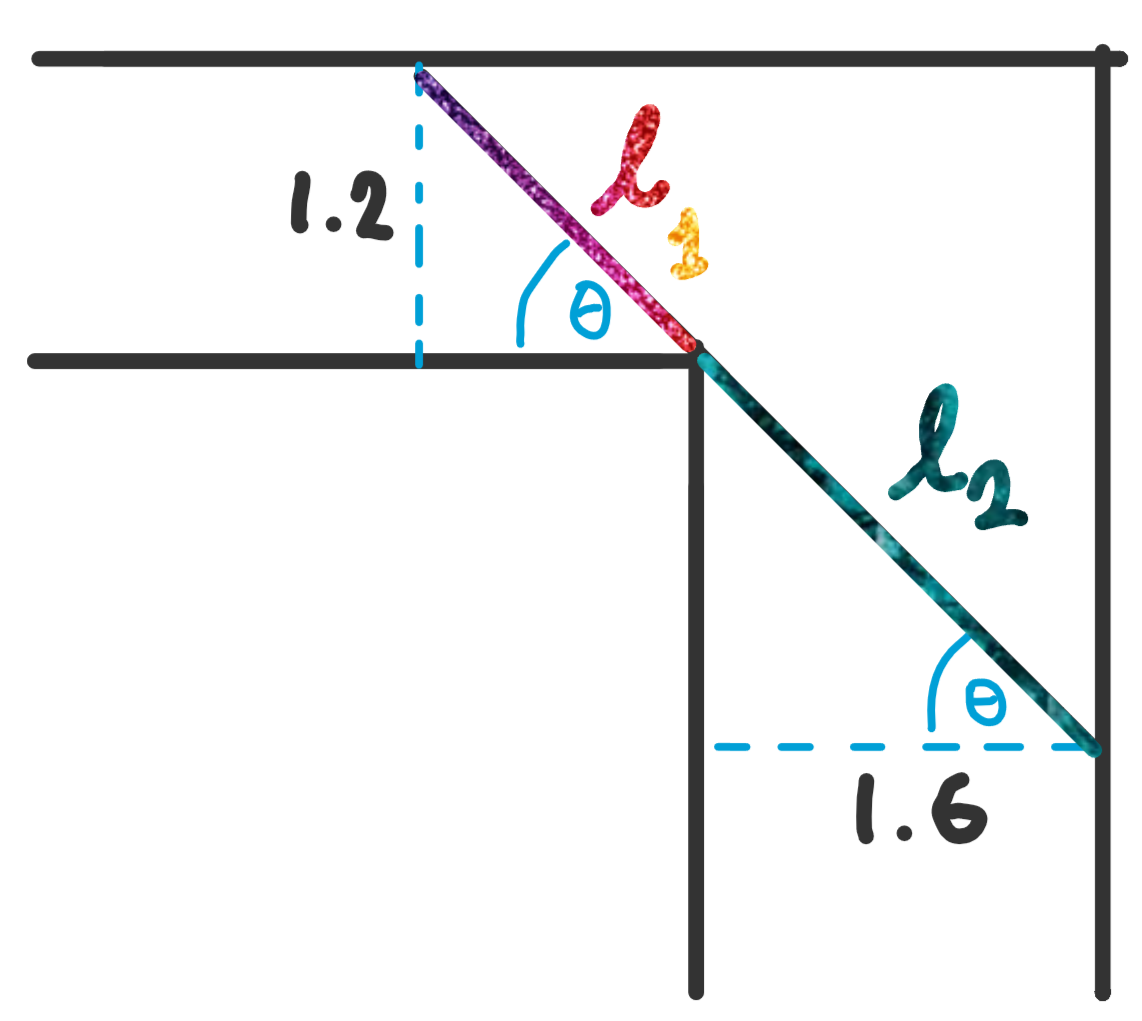
\includegraphics[width=\textwidth]{imgs/op1.png}
\end{minipage}%
\begin{minipage}{0.5\textwidth}
\begin{align*}
    L &= \ell_1 + \ell_2 \\
    L(\theta) &= \frac{1.2}{\sin \theta} + \frac{1.6}{\sin \theta} \\
              &= 1.2(\sin \theta)^{-1} + 1.6(\cos \theta)^{-1} \\
    L'(\theta) &= 1.2(\sin \theta)^{-2} + 1.6(\cos \theta)^{-2} \\
    L'(\theta) &= 0 \implies \textcolor{red}{-1.2(\sin \theta)^{-2}(\cos \theta)} - \textcolor{blue}{1.6(\cos \theta)^{-2}(-\sin \theta)} \\
\end{align*}
\end{minipage}

\begin{align*}
    & \textcolor{red}{\underbrace{\frac{-1.2(\cos \theta )}{(\sin \theta)^2}}} + \textcolor{blue}{\underbrace{\frac{1.6 \cos \theta }{(\cos \theta)^2}}} = 0 \\
    & \frac{1.6 \cos \theta }{(\cos \theta)^2} = \frac{1.2(\cos \theta )}{(\sin \theta)^2} \\
    & 1.6 \sin^3\theta = 1.2 \cos ^3 \theta \\
    & \frac{1.6 \sin^3 \theta}{\cos ^3\theta} = 1.2 \\
    & \frac{\sin^3 \theta}{\cos ^3\theta} = \frac{1.2}{1.6} \\
    & \left(\frac{\sin \theta }{\cos \theta}\right)^3 = \frac{1.2}{1.6} \\
    & (\tan)^3 = \sqrt[3]{\frac{1.2}{1.6}} \\
    & \theta \approx 42.26^{\circ}
\end{align*}
\[
L(42.26) = \frac{1.2}{\sin 42.26^{\circ}} \approx 3.95. \quad \therefore \text{max length is 3.95m.}
\]
\newpage
\subsubsection*{Example 2:}
Joey needs a ladder to break out of prison. He will lean the ladder against a tall fence, over the top of a 5 m high wall that is 3 m from the tall fence. He hopes to climb diagonally along the ladder, over the wall, to the fence. Then he climbs up and over the fence and escapes.\\
What is the minimum length of ladder necessary? No domain is necessary? 


\begin{minipage}{0.5\textwidth}
  \centering
  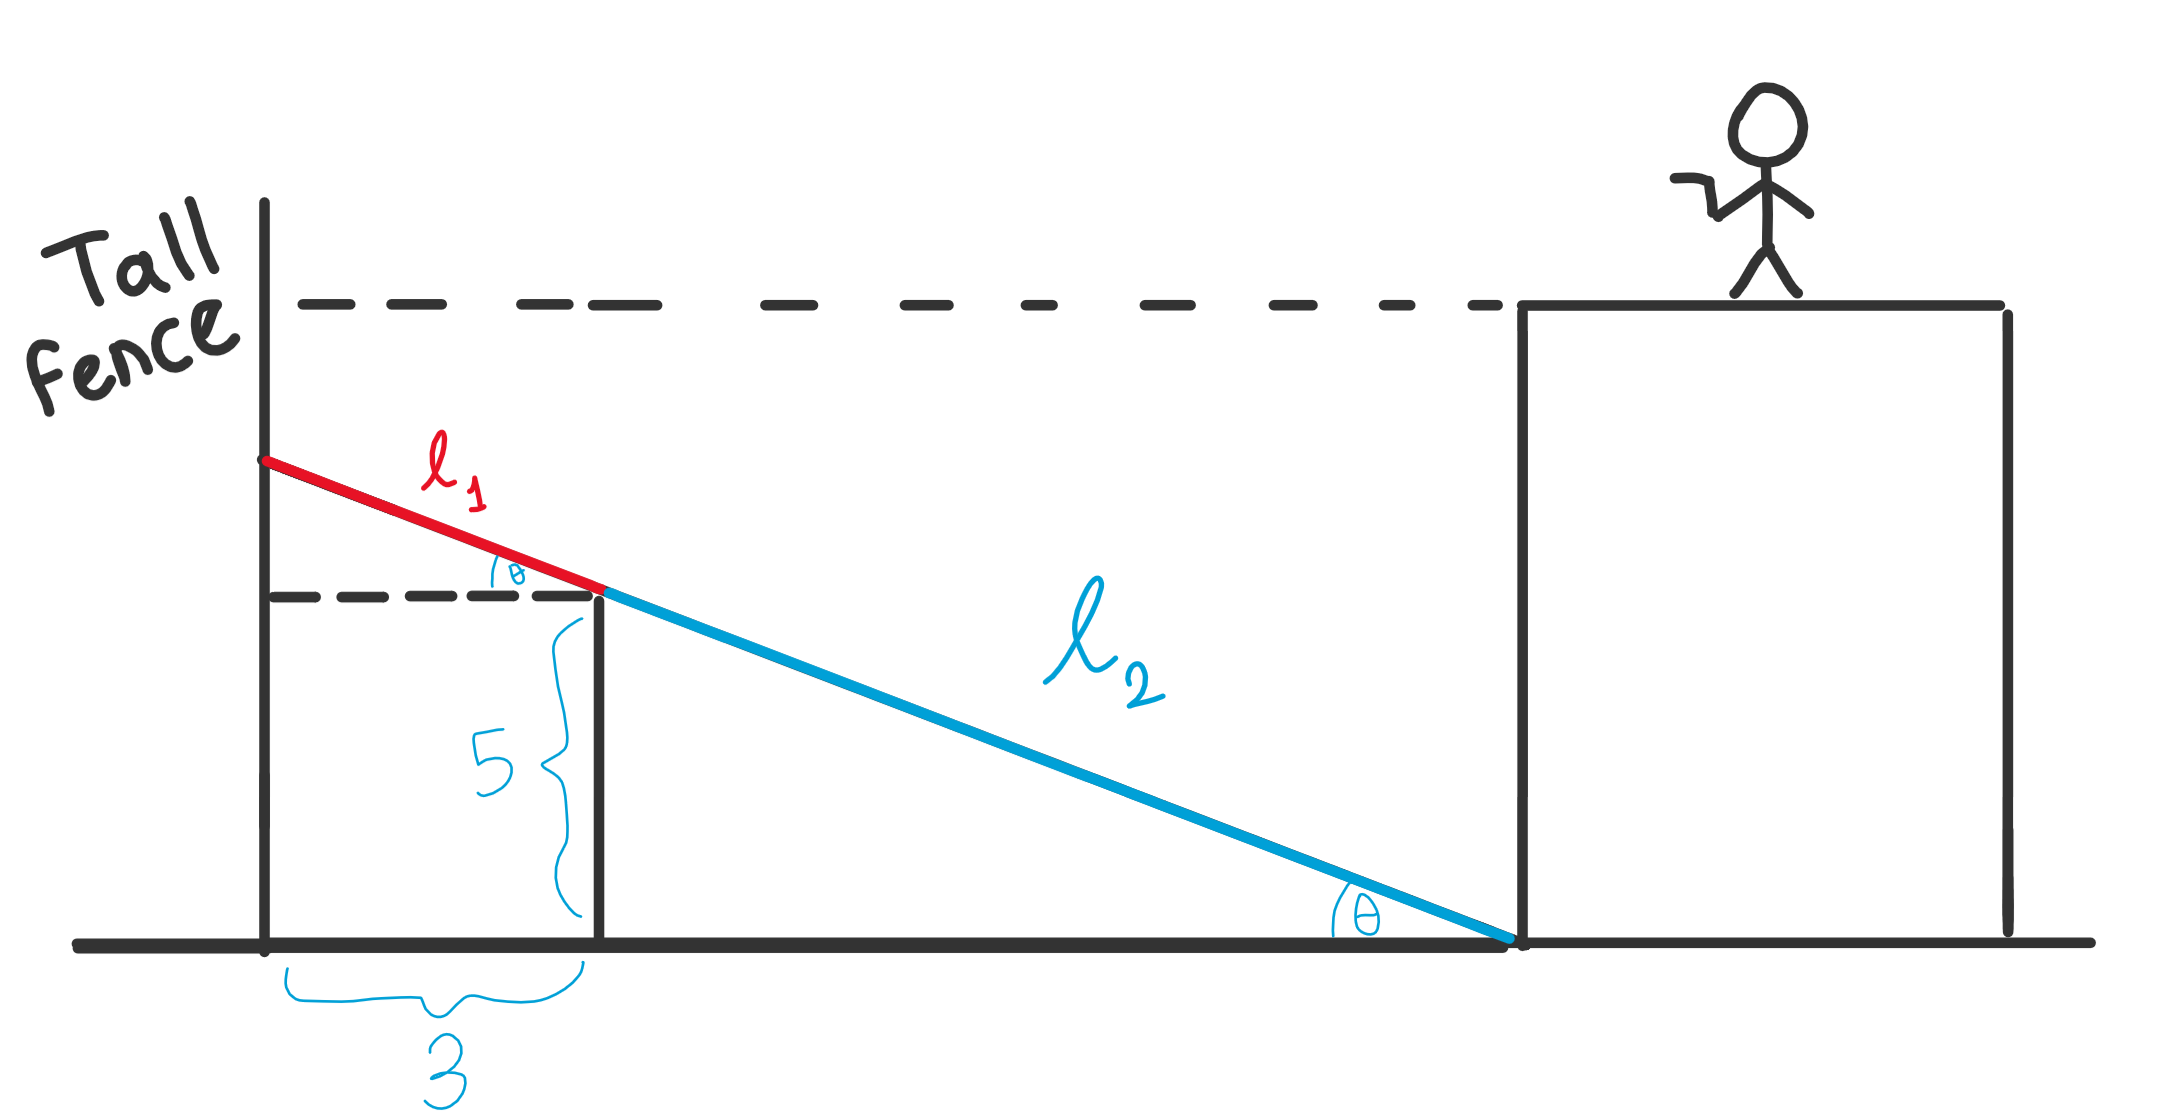
\includegraphics[width=\textwidth]{imgs/op2.png}
\end{minipage}%
\begin{minipage}{0.5\textwidth}
    \begin{align*}
        &L=\ell_1+\ell_2\\
        &L(\theta)=3(\cos\theta)^{-1}+5(\sin \theta)^{-1}\\
        &L'(\theta)=0 \implies \textcolor{red}{-3(\cos\theta)^{-2}(-\sin\theta)}-\textcolor{blue}{5(\sin \theta)^{-2}(\cos \theta)=0}
    \end{align*}
\end{minipage}
\begin{align*}
    &\frac{3\sin\theta}{\cos^2\theta}-\frac{-5\cos \theta}{\sin^2\theta}=0\\
    &\frac{3\sin \theta}{\cos^2\theta}=\frac{5\cos \theta}{\sin^2\theta}\\
    &3\sin^3\theta=5\cos^3\theta\\
    &\frac{\sin^3\theta}{\cos^3\theta}=\frac{5}{3}\\
    &\tan^3=\frac{5}{3}\\
    &\tan^3=\sqrt[3]{\frac{5}{3}}\\
    &\theta \approx49.85^{\circ}\\
\end{align*}
$$L(49.85^{\circ})=\frac{3}{\cos(49.85)}+\frac{5}{\sin(49.85)}\approx 11.2. \therefore \text{laddin must be at least 11.2m long} $$
\newpage 
\subsection{Trig Optimization Word Problem 2}
\subsubsection*{Example 1: }
Determine the greatest possible area of the trapezoid shown below; you are given three side lengths and the top side is as long as you need it to be.

\begin{minipage}{0.5\textwidth}
  \centering
  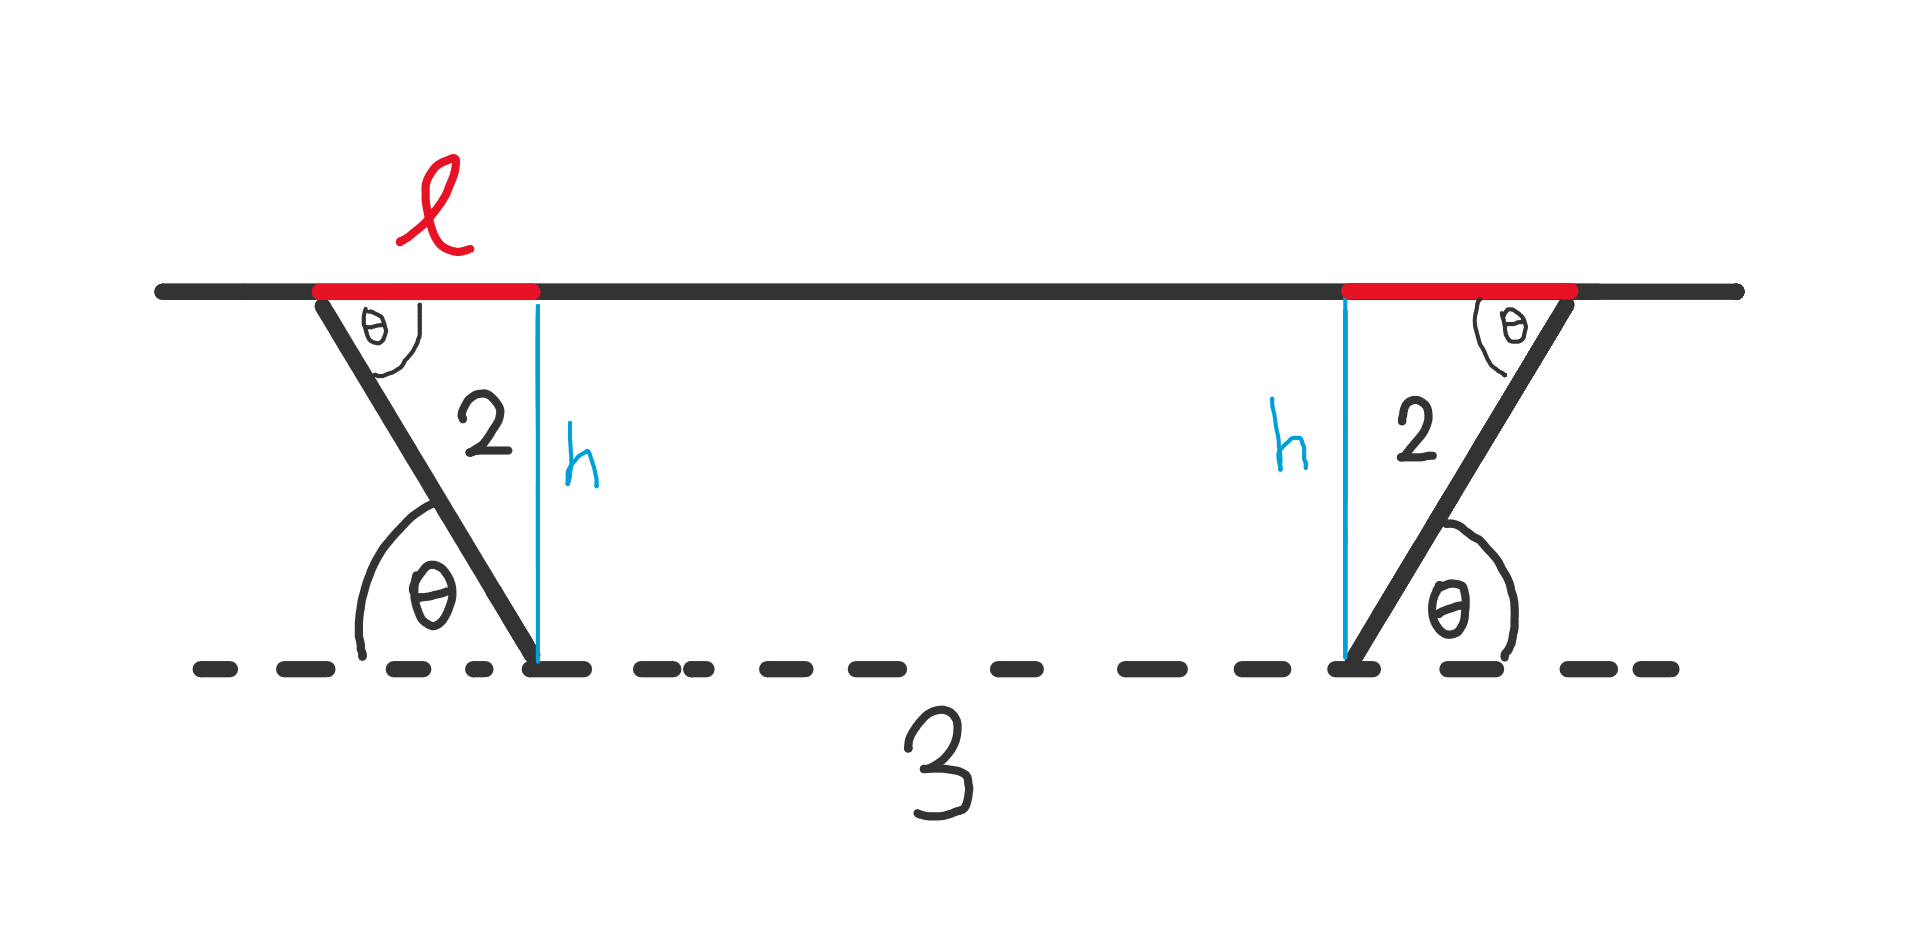
\includegraphics[width=\textwidth]{imgs/op3.png}
\end{minipage}%
\begin{minipage}{0.7\textwidth}
    \begin{align*}
        &\text{Area = }\text{(Area of $\Delta$)}(2)+ \ell \omega\\
        &\sin \theta=\frac{h}{2} \quad \cos \theta= \frac{\ell}{2}\\
        &h=\frac{2}{\sin\theta} \quad \boxed{\ell=2\cos\theta}\\
        &\boxed{h=2\sin\theta}
    \end{align*}
\end{minipage}
\begin{align*}
    &=\frac{1}{2}\left[2(\cos\theta)(2\sin\theta)(2)+3(2\sin\theta)\right]\\
    &A(\theta)=4\sin \theta\cos\theta+6\sin\theta\\
    &A'(\theta)=4\cos\theta\cos \theta + 4 \sin \theta(-\sin \theta)+6\cos \theta\\
    &A'(\theta)=0 \implies 4\cos^2 \theta -4\sin^2 \theta +6 \cos \theta=0\\
    &4 \cos^2-4(1-\cos ^2\theta)+6\cos \theta=0\\
    &4\cos^2\theta-4+4\cos^2\theta+6\cos \theta=0\\
    &8\cos^2\theta+6\cos -4=0\\
    &\cos \theta=\frac{=6\pm \sqrt{36+128}}{16}\\
    &0.425 \quad \text{or} \quad \cancel{-1.1753}\\
    &\cos^{-1}(0.425)\approx 64.8^{\circ}\\
\end{align*}
$$A(64.8^{\circ})=4\sin(64.8^{\circ})\cos(64.8^{\circ})+6\sin(64.8^{\circ})\approx6.97$$
\subsection{Derivatives of Exponential Functions}
Three key rules for this section are\\
\begin{itemize}
    \item The derivative of $\lm x$ with respect to $x$ is $\frac{1}{x}$
    \item The derivative of $e^x$ with respect to $x$ is $e^x$
    \item The derivative of $b^x$ with respect to $x$ is $(b^x)(\ln b)$
\end{itemize}

Putting the last rule together with the chain rule, we get that
$$\text{Derivative of } b^{f(x)} \text{is } b^{f(x)}(\ln n)f'(x)$$
\begin{tcolorbox}[colback=blue!5!snow, colframe=white!50!white,
  colbacktitle=blue!75!mistyrose, title=Derivatives of Exponential Functions Rules]
    \begin{align*}
        \frac{\delta(\ln x)}{\delta x}&=\frac{1}{x}\\
        \frac{\delta(e^x)}{\delta x}&=e^x\\
        \frac{\delta (b^x)}{\deleta x}&= b^{x}(\ln b)\\
        \frac{\delta (b^{f(x)})}{\delta x}&=b^{f(x)}\ln b f'(x)\\
    \end{align*}  
\end{tcolorbox}
In other words, to differentiate an exponential function, restate the function, multiply by the natural logarithm (ln) of the base, and then multiply by the derivative of the exponent. This is assuming that there is no $x$ in the base as well. We will see that there is a different process when there is an $x$ in both the base and in the exponent.

\subsubsection*{Example 1:}
Determine the derivative of $g(x)=e^{x^2-x}$
\subsubsection*{Solution: }
$g'(x)=e^{x^2-x}(2x-1)$
\subsubsection*{Example 2:}
Determine the derivative of the curve $f(x)=x^2e^x$
\subsubsection*{Solution:}
$f'(x)=2xe^e+x^2e^x$
\subsubsection*{Example 3:}
Determine the equation of the tangent line to $y=\frac{e^x}{x^2}$ where $x=1$.
\subsubsection*{Solution: }
at $x=1$, $y=\frac{e^1}{(1)^2}=\frac{e}{1} \quad (1, e)$ this is called the points.\\
The slope is:
$$y'=\frac{x^2e^x-e^x(2x)}{x^4}$$
$\therefore \text{at } x=1, y'=\frac{(1)^2e^1(2(1))}{(1)^4}= \frac{e-2e}{1}=-e$ \\
The question is not over yet, we need to solve the tangent of equation by using some skills from grade 9th math. Therefore:
\begin{align*}
    y&=mx+b\\
    y&=-ex+b\\
    &\text{plug in (1, e)}\\
    e&=-e(1)+b\\
    2e&=b
\end{align*}
$\therefore$ the equation of the tangent line is $y=-ex+2e$
\subsubsection*{Example 4:}
Differentiate the function $f(x)=5x^x$
\subsubsection*{Solution: }
$f'(x)=5^x(\ln 5)$
\subsubsection*{Example 5:}
Differentiate the function $h(x)=(8)7^{9x^2-5x+1}$
\subsubsection*{Solution: }
$h'(x)=(8)7^{9x^2-5x+1}(\ln 7)(18x-5)$

\subsubsection*{Word Problem 1:}
On January 1, 1850, the population of Goldrushtown was 50000. Since then the population of Goldrushtown can be expressed as $P(x)=50000(0.98)^t$.
\begin{enumerate}
    \item[a)] What was the population of Goldrushtown on January 1, 1900?
    \item{b)} At what rate was the population changing on January 1, 1900? 
\end{enumerate}
\subsubsection*{Solution: }
\begin{enumerate}
    \item[a)] $P(50)=50000(0.98)^{50} \approx 18208$
    \item[b)] 
    \begin{align*}
        P(x)&=50000(0.98)^t\\
        P'(x)&=50000(0.98)^t(\ln 0.98)\\
        P'(50)&=50000(0.98)^{50}(\ln 0.98)\\
        &\approx-367.8 = -368
    \end{align*} 
$\therefore$ the population is decreasing at rate of approximately 368 people per year.    
\end{enumerate}
\subsubsection*{Word Problem 2:}
A radioactive substance decays exponentially. The percent, P, of the material left after after t years is $P(t)=100(1.015)^{-t}$
\begin{enumerate}
    \item[a)] What is the half-life?
    \item[b)] How fast is the substance decaying at that time?
\end{enumerate}
\subsubsection*{Solution: }
\begin{enumerate}
    \item[a)]
    \begin{align*}
        50 &= 100 \times (1.015)^{-t}\\
        \frac{50}{100} &= (1.015)^{-t}\\
        \frac{1}{2} &= (1.015)^{-t}\\
        -t &= \log_{1.015}\left(\frac{1}{2}\right)\\
        -t &= \frac{\log\left(\frac{1}{2}\right)}{\log(1.015)}\\
        t &\approx 46.59
    \end{align*}
    $\therefore$ the lalf-life is approximately 47 years.
    \item[b)] 
    \begin{align*}
        P'(x)&=100(1.015)^{-t}\ln (1.015)\\
        P'(47)&=100(1.015)^{-47}\ln (1.015)\\
        &\approx 0.74
    \end{align*} 
    $\therefore$ at that time, the population is decreasing at the rate of 0.76\% of the original amount per year.
\end{enumerate}
\newpage 
\subsection{Optimization Involving Exponential Functions}
\subsubsection*{Example 1:}
The effectiveness of studying for an exam depends on how many hours a student studies. Some experiments show that if the effectiveness, E is put on a scale from 0 to 10, then
$$E(t)=0.5\left[10+te^{\frac{-t}{20}}\right]$$
where t is the number of hours spent studying for an examination. If a student has up to 30 hours for studying, how many hours are needed for maximum effectiveness?
\begin{align*}
    &=5+0.5t^{\frac{-t}{20}}\\
    E(t)=0 \implies & 0.5e^{-\frac{1}{20}t}+0.5te^{-\frac{1}{20}} \left(-\frac{1}{20}\right)=0\\
    &\underbrace{0.5e^{-\frac{1}{20}t}}_{\text{cannot equal to 0}} \underbrace{\left(1-\frac{1}{20}t\right)}_{\downarrow }=0\\
    &\quad \quad 1-\frac{1}{20}t=0 \implies 1=\frac{1}{20}t\\
    &\quad \quad \quad 20=t
\end{align*}
Now, we need to use the domain analysis:

\begin{align*}
    E(0)&=5+0.5(0)e^{-\frac{1}{20}}=5\\
    E(20)&\approx8.68\\
    E(30)&\approx8.35
\end{align*}
$\therefore$ the maximum effectiveness satvik should study 20 hours.
\newpage 

\subsubsection*{Example 2:}
A consultant determines that the proportion of people who have responded to the advertisement of a new product after it has been marketed for t days is given by $f(t)=0.7(1-e^{-0.2t})$.The area covered by that advertisement contains 10 million potential customers and each response to the ad yields revenue of \$0.70 on average (excluding the cost of advertising). The ad costs \$30000 to produce and a further \$5000 per day to run.

\begin{enumerate}
    \item[a)] Determine $\lim_{t\to\infty}f(t)$ and interpret the result.
    \item[b)] What percent of potential customers have responded after 7 days of advertising?
    \item[c)] Write the function P(t) that represents the average profit after t days of advertising. What is the average profit after 7 days?
    \item[d)] For how manyfull days should the ad campaign be run in order to maximize the average profit? Assume an advertising budget of \$200000.
\end{enumerate}
\subsubsection*{Solution: }
\begin{enumerate}
    \item[a)] 
    \begin{align*}
        &0.7-0.7e^{-0.2t}\\
        \lim_{t\to \infty}f(t) &=\lim_{t\to \infty}0.7-\frac{0.7}{e^{0.2t}}\\
        &=0.7
    \end{align*}
$\therefore$ if the ad runs forever, only 7070 of people will respond. 
    \item[b)] $f(7)=0.7-0.7e^{-0.2(7)}\approx 53$
    $\therefore$ after 7 days 539 of population have responded.
    \item[c)] 
    \begin{align*}
    \text{Profit } &= \text{Revenue - Cost}\\    
    \text{Revenue }&=(0.70)\text{(number of responses)}\\
    &=(0.70)\text{(population)(percentage of population who have responded)} \\
    &=(0.70)(1000000)(f(t))\\
    &=70000000\left[(0.7(1-e^{-0.2t}))\right]\\
    &=70000000(0.7-0.7e^{-0.2t})\\
    &=4900000-4900000e^{-0.2t}\\
    \end{align*}
    \begin{align*}
    \text{Cost} &= \text{Production cost + Opening cost}\\
    &=3000+5000\text{(# of days)}\\
    c(t)&=30000+5000t\\
    P(t)&=R(t)-C(t)\\
    &=4900000-4900000e^{-0.2t}-(30000+5000t)\\
    &=4870000-4900000e^{-0.2t}-500t\\
    P(7)&=4870000-490000e^{-0.2(7)}-5000(7)\\
    &\approx 3626674.88
    \end{align*}
    \item[d)] 
    \begin{align*}
        \text{Domain Work}\\
        t &\geq 0\\
        \text{Cost} &\leq 200000\\
        300000+5000+&\leq 20000\\
        5000t&\leq 170000\\
        t&\geq34\\
        \therefore 0\leq &t \leq 34
    \end{align*} 
    \begin{align*}
        P'(t) 0\implies -4900000e^{-0.2t}(-0.2)-5000&=0\\
        98000e^{-0.2t}&=5000\\
        e^{-0.2t}&=\frac{5000}{98000}\\
        -0.2t&=\ln \left(\frac{5000}{980000}\right)\\
        t&=\frac{\ln \left(\frac{5000}{980000}\right)}{-0.2} \approx 26
    \end{align*}
    \begin{align*}
        P(0)&=487000-4900000e^{-0.2}-5000(0)=-30000\\
        P(26)&=4712968.83\\
        P(34)&=4694542.50
    \end{align*}
    $\therefore$ max profit at 26 days
\end{enumerate}
\newpage 
\subsection{Logarithmic Differentiation}
We know how to find the derivative of a power of x. For example, if we are given the function $y=3x^2$, we see that x is in the base of the exponent and we know that we can use the power rule.\\
We also know how to find the derivative of an exponential function, where x is in the exponent. For example, if we are given the function $y=3^{2x-1}$, we see that x is in the exponent and we can use exponential differentiation.\\
But what do we do if we have a function where x is in the base of the exponent and in the exponent. For example, how would we determine the derivative of the function $y=x^x$. \\
If we have a power with x in both the base of the exponent and in the exponent itself, we can determine the derivative by taking the natural logarithm (i.e., ln) of both sides, then using previously learned rules of derivatives such as implicit differentiation and the power rule, among others, to isolate $y'$ and thus determine the derivative

\subsubsection*{Example 1:}
Determine the derivative with respect to x of $y=x^x$.
\subsubsection*{Solution: }
\begin{align*}
    \log &= \ln x^x\\
    \ln y &=x\ln x\\
    \frac{1}{y} \frac{\delta y}{\delta x} &=\ln x +x\left(\frac{1}{x}\right)\\
    \frac{1}{y} \frac{\delta y}{\delta x} &=\ln x+1\\
    \frac{\delta y}{\delta x}&=x^x(\ln x+1)
\end{align*}
\subsubsection*{Example 2:}
Determine the derivative with respect to x of $y=(3x+4)^{x^4-2x}$
\subsubsection*{Solution: }
\begin{align*}
    \ln y &=\ln (3x+4)^{x^4-2x}\\
    \ln y &=(x^4-2x) \ln(3x+4)\\
    \frac{1}{y}\frac{\delta y}{\delta x}&=(4x^3-2)\ln(3x+4)+(x^4-2x)\left(\frac{1}{3x+4}\right)(3)   
\end{align*}
    \text{or}
    \begin{align*}
    \frac{\delta y}{\delta x}&=y\left[(4x^3-2)\ln(3x+4)+\frac{(x^4-2x)(3)}{3x+4}\right]\\
    \frac{\delta y}{\delta x}&=(3x+4)^{x^4-2x}\left[(4x^3-2)\ln(3x+4)+\frac{(x^4-2x)(3)}{3x+4}\right]\\ 
    \end{align*}
    Sometimes Logarithmic differentiation can be used to answer other questions where it might not necessarily be applicable.
    We will prove the power rule using Logarithmic differentiation in a moment, and then we will do an example where Logarithmic differentiation is beneficial to a question that would otherwise be rather complicated.
\subsubsection*{Example 3:}
    Using logarithmic differentiation, prove the power rule; i.e prove that if $f(x)=x^n$, then $f'(x)=nx^{n-1}$
\subsubsection*{Solution: }

First, take the natural logarithm of both sides:

$$\ln(f(x)) = \ln(x^n)$$

Using the property of logarithms that allows us to bring the exponent down as a coefficient, we get:

$$\ln(f(x)) = n \cdot \ln(x)$$

Now, differentiate both sides with respect to $x$. On the left side, we use the chain rule, and on the right side, the derivative of $\ln(x)$:

$$\frac{1}{f(x)} \cdot f'(x) = n \cdot \frac{1}{x}$$

Solving for $f'(x)$ gives us:

$$f'(x) = f(x) \cdot n \cdot \frac{1}{x}$$

Since $f(x) = x^n$, we substitute $f(x)$ back in:

$$f'(x) = x^n \cdot n \cdot \frac{1}{x}$$

Simplify the expression by canceling one $x$ from $x^n$ and $x$ in the denominator:

$$f'(x) = n \cdot x^{n-1}$$

And there we have it, the power rule is proven using logarithmic differentiation:

$$f'(x) = nx^{n-1}$$

This shows that the derivative of $x^n$ with respect to $x$ is indeed $nx^{n-1}$.

\subsubsection*{Example 4:}
Use logarithmic differentiation to evaluate $\frac{\delta y}{\delta x}$ at $x=-1$ $$y=\frac{(x^4+1)\sqrt{x+2}}{2x^2+2x+1}$$
\subsubsection*{Solution:}

 $$y=\frac{(x^4+1)\sqrt{x+2}}{2x^2+2x+1}$$ at $x=-1$ using logarithmic differentiation, follow these steps:

1. Take the natural logarithm of both sides of the equation to obtain an expression that can be differentiated implicitly:
   $$\ln(y) = \ln\left(\frac{(x^4+1)\sqrt{x+2}}{2x^2+2x+1}\right)$$

2. Simplify the right-hand side using the properties of logarithms:
   $$\ln(y) = \ln(x^4+1) + \frac{1}{2}\ln(x+2) - \ln(2x^2+2x+1)$$

3. Differentiate both sides with respect to $x$:
   $$\frac{1}{y}\frac{\delta y}{\delta x} = \frac{4x^3}{x^4+1} + \frac{1}{2(x+2)} - \frac{4x+2}{2x^2+2x+1}$$

4. Multiply through by $y$ to solve for $\frac{dy}{dx}$:
   $$\frac{\delta y}{\delta x} = y\left(\frac{4x^3}{x^4+1} + \frac{1}{2(x+2)} - \frac{4x+2}{2x^2+2x+1}\right)$$

5. Substitute $y$ with the original function:
   $$\frac{\delta y}{\delta x} = \frac{(x^4+1)\sqrt{x+2}}{2x^2+2x+1}\left(\frac{4x^3}{x^4+1} + \frac{1}{2(x+2)} - \frac{4x+2}{2x^2+2x+1}\right)$$

6. Now, evaluate the derivative at $x=-1$:
   $$\frac{\delta y}{\delta x}\bigg|_{x=-1} = \frac{((-1)^4+1)\sqrt{-1+2}}{2(-1)^2+2(-1)+1}\left(\frac{4(-1)^3}{(-1)^4+1} + \frac{1}{2(-1+2)} - \frac{4(-1)+2}{2(-1)^2+2(-1)+1}\right)$$

7. Simplify the expression:
   $$\frac{\delta y}{\delta x}\bigg|_{x=-1} = \frac{(1+1)\sqrt{1}}{2+2(-1)+1}\left(\frac{-4}{1+1} + \frac{1}{2(1)} - \frac{-4+2}{2+2(-1)+1}\right)$$
   $$\frac{dy}{dx}\bigg|_{x=-1} = \frac{2}{1}\left(\frac{-4}{2} + \frac{1}{2} - \frac{-2}{1}\right)$$
   $$\frac{dy}{dx}\bigg|_{x=-1} = 2\left(-2 + \frac{1}{2} + 2\right)$$
   $$\frac{dy}{dx}\bigg|_{x=-1} = 2\left(\frac{1}{2}\right)$$
   $$\frac{dy}{dx}\bigg|_{x=-1} = 1$$

Therefore, the derivative of the function at $x=-1$ is $1$.\\
Another time when we use logarithmic differentiation is when we are given a logarithmic function in a base other than e(i.e, when we are not using the natural logarithmic $\ln$).\\\\
We will see that in these cases, we convert our logarithmic function to the equivalent equation and then use the natural logarithmic.
\subsubsection*{Example 5: }
Determine $\frac{\delta y}{\delta x}$ given that $y=\long_3(4x^2-5x+1)$
\subsubsection*{Solution: }
\begin{align*}
    3^y&=4x^2-5x+1\\
    \log 3^y&=\ln(4x^2-5x+1)\\
    y\log_3&=\ln(4x^2-5x+1)\\b
    y&=\left(\frac{1}{\ln 3}\right)\ln(4x^2-5x+1)\\
    \frac{\delta y}{\delta x}&=\left(\frac{1}{\ln 3}\right)\left(\frac{1}{4x^2-5x+1}\right)(8x-5)\\
    &=\frac{8x-5}{\ln(4x^2-5x+1)}
\end{align*}
\end{document}